\documentclass[aspectratio=169,11pt]{beamer}

\usetheme{metropolis}
\usepackage[table]{xcolor}
\usepackage{booktabs}
\usepackage{tikz}
\usepackage{amsmath}
\usepackage{array}
\usepackage{caption}
\usepackage{tcolorbox}
\usepackage[T1]{fontenc}
\usepackage{lmodern}
\usepackage{fontawesome5}
\tcbuselibrary{skins, raster}
\usetikzlibrary{positioning, arrows.meta, shapes.geometric, calc, shadows.blur, backgrounds}

% Palette
\definecolor{ink}{HTML}{0B2838}        % deep teal-navy
\definecolor{inkdeep}{HTML}{06181F}    % darker
\definecolor{amber}{HTML}{F2A340}      % warm amber
\definecolor{emerald}{HTML}{2DA86F}    % accent emerald
\definecolor{coral}{HTML}{E45F56}      % alert
\definecolor{paper}{HTML}{F8F4EB}      % cream
\definecolor{soft}{HTML}{EAE4D4}       % muted card bg
\definecolor{rule}{HTML}{D2C9B4}       % rule lines
\definecolor{muted}{HTML}{7F756A}      % body grey
\definecolor{ash}{HTML}{4A4A4A}        % strong body

\setbeamercolor{normal text}{fg=ink, bg=paper}
\setbeamercolor{background canvas}{bg=paper}
\setbeamercolor{alerted text}{fg=coral}
\setbeamercolor{example text}{fg=emerald}
\setbeamercolor{frametitle}{fg=paper, bg=ink}
\setbeamercolor{title}{fg=paper}
\setbeamercolor{subtitle}{fg=paper}
\setbeamercolor{author}{fg=paper}
\setbeamercolor{progress bar}{fg=amber, bg=soft}
\setbeamercolor{block title}{fg=paper, bg=emerald}
\setbeamercolor{block body}{fg=ink, bg=soft}
\setbeamercolor{block title alerted}{fg=paper, bg=coral}
\setbeamercolor{block body alerted}{fg=ink, bg=soft}
\setbeamercolor{block title example}{fg=paper, bg=emerald}
\setbeamercolor{block body example}{fg=ink, bg=soft}
\setbeamerfont{frametitle}{size=\large, series=\bfseries}
\setbeamerfont{title}{size=\Huge, series=\bfseries}
\setbeamertemplate{itemize item}{\color{amber}\faIcon{angle-right}}
\setbeamertemplate{itemize subitem}{\color{emerald}\faIcon{angle-right}}
\setbeamertemplate{section in toc}{\inserttocsectionnumber. \inserttocsection}

% Reusable tcolorbox style
\newtcolorbox{factbox}[1][]{
  enhanced, colback=soft, colframe=amber, boxrule=0pt,
  leftrule=4pt, arc=2pt, top=4pt, bottom=4pt, left=8pt, right=8pt,
  fontupper=\small, before skip=4pt, after skip=4pt, #1}
\newtcolorbox{alertbox}[1][]{
  enhanced, colback=soft, colframe=coral, boxrule=0pt,
  leftrule=4pt, arc=2pt, top=4pt, bottom=4pt, left=8pt, right=8pt,
  fontupper=\small, before skip=4pt, after skip=4pt, #1}
\newtcolorbox{teabox}[1][]{
  enhanced, colback=soft, colframe=emerald, boxrule=0pt,
  leftrule=4pt, arc=2pt, top=4pt, bottom=4pt, left=8pt, right=8pt,
  fontupper=\small, before skip=4pt, after skip=4pt, #1}

% Custom title chip
\newcommand{\chip}[2][amber]{%
  \tikz[baseline=(c.base)]\node[fill=#1, text=ink, rounded corners=3pt,
                                  inner xsep=6pt, inner ysep=3pt,
                                  font=\bfseries\small] (c) {#2};}

\title{CHRONO-Fair}
\subtitle{Time-Resolved Counterfactual Fairness Monitoring \\ for Clinical Machine Learning}
\author{Supervisor planning meeting \\ \footnotesize Anonymous draft, in-progress research}

\begin{document}

% ==========================================================
% Slide 1: Title (custom tikz)
% ==========================================================
{
\setbeamercolor{background canvas}{bg=ink}
\begin{frame}[plain,noframenumbering]
\begin{tikzpicture}[remember picture, overlay]
  % accent shapes
  \fill[amber, opacity=0.15] (current page.north east) circle (5cm);
  \fill[emerald, opacity=0.10] (current page.south west) circle (5cm);
  \draw[amber, line width=2.5pt] ([xshift=1.4cm,yshift=-1.2cm]current page.north west) -- ++(2.5,0);
  % title
  \node[anchor=north west, text=amber, font=\bfseries\large]
       at ([xshift=1.4cm,yshift=-1.6cm]current page.north west)
       {SUPERVISOR PLANNING MEETING};
  \node[anchor=north west, text=paper, font=\fontsize{44}{50}\bfseries\selectfont]
       at ([xshift=1.4cm,yshift=-2.6cm]current page.north west)
       {CHRONO-Fair};
  \node[anchor=north west, text=paper, font=\Large]
       at ([xshift=1.4cm,yshift=-4.4cm]current page.north west)
       {Time-Resolved Counterfactual Fairness Monitoring};
  \node[anchor=north west, text=paper, font=\Large]
       at ([xshift=1.4cm,yshift=-5.0cm]current page.north west)
       {for Clinical Machine Learning};
  \node[anchor=north west, text=soft, font=\large\itshape]
       at ([xshift=1.4cm,yshift=-6.0cm]current page.north west)
       {Extends our prior VFR-Audit three-axis static auditing framework};
  \node[anchor=north west, text=soft, font=\normalsize]
       at ([xshift=1.4cm,yshift=-6.6cm]current page.north west)
       {Target venue: Q1 digital-health / health-informatics journal};
  \draw[amber, line width=1pt] ([xshift=1.4cm,yshift=-7.3cm]current page.north west) -- ++(2.8,0);
  \node[anchor=north west, text=soft, font=\footnotesize\itshape]
       at ([xshift=1.4cm,yshift=-7.5cm]current page.north west)
       {Anonymous draft \textbar\ in-progress research \textbar\ not finalised};
\end{tikzpicture}
\end{frame}
}

% ==========================================================
% Slide 2: Where clinical ML stands
% ==========================================================
\begin{frame}{Where clinical ML stands today}
\small
\begin{factbox}
\faIcon{stethoscope}\enspace Clinical ML supports triage, risk scoring, and length-of-stay prediction across many sites~[1, 2].
\end{factbox}
\begin{alertbox}
\faIcon{exclamation-triangle}\enspace Documented post-release subgroup failures across radiology, sepsis, kidney function, and care-allocation models~[3, 4, 5, 6].
\end{alertbox}
\begin{teabox}
\faIcon{landmark}\enspace Regulatory expectations have shifted toward continuous lifecycle monitoring~[7, 8] with reporting standards~[9, 10, 11, 12].
\end{teabox}
\begin{factbox}
\faIcon{tools}\enspace Auditing toolkits in routine use return a thresholded pass-or-fail verdict on a fixed snapshot~[13, 14, 15, 16].
\end{factbox}
\vspace{2pt}
\centering\textbf{\color{ink}\large That verdict is the object hospitals act on. The snapshot tells us nothing about its stability over time.}
\end{frame}

% ==========================================================
% Slide 3: Prior VFR-Audit
% ==========================================================
\begin{frame}{Our prior VFR-Audit study \hfill \chip[soft]{static auditing framework}}
\vspace{2pt}
\textbf{Three audit-reliability axes on real Texas-100X (925\,128 records) [17]:}
\vspace{2pt}
\begin{itemize}
\setlength\itemsep{0pt}
\item[\faIcon{circle-notch}] Axis 1: resampling fluctuation of the fairness verdict.
\item[\faIcon{compress-arrows-alt}] Axis 2: audit-size sensitivity of the fairness verdict.
\item[\faIcon{hospital}] Axis 3: cross-hospital-site agreement of the fairness verdict.
\end{itemize}
\vspace{4pt}
\textbf{Standard vs Fair monitored-model setup (cited from prior work):}
\vspace{2pt}
\centering
\small
\setlength{\arrayrulewidth}{0.8pt}
\arrayrulecolor{rule}
\begin{tabular}{>{\bfseries}l c c c}
\toprule
\rowcolor{ink}
{\color{paper}\textbf{Attribute}} & {\color{paper}\textbf{Std DI}} & {\color{paper}\textbf{Fair DI}} & {\color{paper}\textbf{Verdict}} \\
\midrule
Race      & 0.654 & \cellcolor{soft}\textbf{0.884} & \color{coral}fail $\rightarrow$ \color{emerald}\textbf{pass} \\
Sex       & 0.762 & \cellcolor{soft}\textbf{0.933} & \color{coral}fail $\rightarrow$ \color{emerald}\textbf{pass} \\
Ethnicity & 0.832 & \cellcolor{soft}\textbf{0.962} & \color{emerald}pass $\rightarrow$ \color{emerald}\textbf{pass} \\
Age Group & 0.291 & \cellcolor{soft}\textbf{0.801} & \color{coral}fail $\rightarrow$ \color{emerald}\textbf{pass} \\
\bottomrule
\end{tabular}
\vspace{2pt}\\
{\footnotesize\color{muted} Std Acc 0.8777 $\rightarrow$ Fair Acc 0.8248 (reduction of 5.28 pp). Predecessor, not a CHRONO-Fair contribution.}
\end{frame}

% ==========================================================
% Slide 4: Gap
% ==========================================================
\begin{frame}{The remaining gap}
\begin{alertbox}
\faIcon{bullseye}\enspace \textbf{Real Texas-100X anchor finding (925\,128 records) [17].} The worst-group true-positive-rate verdict for race reads ``fair'' at \textbf{0.824}. The same verdict flips to ``unfair'' in \textbf{4 of 20} hospital-network resamples (Verdict Flip Rate \textbf{0.20}). A batch audit cannot tell when, or whether, that verdict reversal recurs as new patients arrive.
\end{alertbox}
\vspace{2pt}
\centering
\small
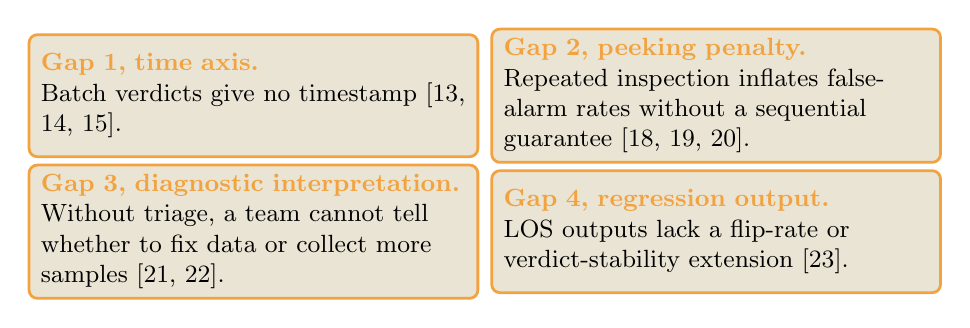
\begin{tikzpicture}[node distance=2pt and 4pt]
\node[draw=amber, line width=1pt, fill=soft, rounded corners=3pt, minimum width=5.7cm, minimum height=1.55cm, align=left, text width=5.4cm, font=\small] (g1) {%
\textbf{\color{amber}Gap 1, time axis.}\\ Batch verdicts give no timestamp~[13, 14, 15].};
\node[draw=amber, line width=1pt, fill=soft, rounded corners=3pt, minimum width=5.7cm, minimum height=1.55cm, align=left, text width=5.4cm, font=\small, right=of g1] (g2) {%
\textbf{\color{amber}Gap 2, peeking penalty.}\\ Repeated inspection inflates false-alarm rates without a sequential guarantee~[18, 19, 20].};
\node[draw=amber, line width=1pt, fill=soft, rounded corners=3pt, minimum width=5.7cm, minimum height=1.55cm, align=left, text width=5.4cm, font=\small, below=of g1] (g3) {%
\textbf{\color{amber}Gap 3, diagnostic interpretation.}\\ Without triage, a team cannot tell whether to fix data or collect more samples~[21, 22].};
\node[draw=amber, line width=1pt, fill=soft, rounded corners=3pt, minimum width=5.7cm, minimum height=1.55cm, align=left, text width=5.4cm, font=\small, below=of g2] (g4) {%
\textbf{\color{amber}Gap 4, regression output.}\\ LOS outputs lack a flip-rate or verdict-stability extension~[23].};
\end{tikzpicture}
\end{frame}

% ==========================================================
% Slide 5: Comparison table
% ==========================================================
\begin{frame}{Closest related work, named and positioned}
\centering
\scriptsize
\setlength{\arrayrulewidth}{0.8pt}\arrayrulecolor{rule}
\begin{tabular}{>{\bfseries}p{3.5cm} p{1.6cm} p{4.4cm} p{4.1cm}}
\toprule
\rowcolor{ink}
{\color{paper}\textbf{Tool / work}} & {\color{paper}\textbf{Mode}} & {\color{paper}\textbf{Output}} & {\color{paper}\textbf{Closest gap}} \\
\midrule
Aequitas~[13]                & Batch & Per-attribute parity-ratio report & No streaming alarm \\
\rowcolor{soft} Fairlearn~[14]              & Batch & Group fairness + reduction mitigator & No verdict-flip monitoring \\
AIF360~[15]                  & Batch & ~20 metrics library              & Snapshot only \\
\rowcolor{soft} Microsoft RAI~[16]          & Notebook & Fairlearn + interpret + CF       & Developer review, not governance \\
Davis et al.~[2]             & Quarterly & Subgroup trend, 11 yr VA      & No per-cell sequential alarm \\
\rowcolor{soft} Prediction sensitivity~[22] & Per batch & CF-flip rate scalar           & No alarm rule \\
VFR-Audit (our prior)~[17]   & Static & Verdict Flip Rate scalar         & No time axis \\
\bottomrule
\end{tabular}
\vspace{4pt}\\
{\footnotesize\color{muted}\itshape Anytime-valid machinery exists~[18, 19, 20]. It has not been applied to counterfactual fairness verdicts at intersectional granularity.}
\end{frame}

% ==========================================================
% Slide 6: One-sentence extension
% ==========================================================
{
\setbeamercolor{background canvas}{bg=ink}
\setbeamercolor{frametitle}{fg=amber, bg=ink}
\begin{frame}{\color{paper}Our planned extension, in one sentence}
\vfill
\begin{center}
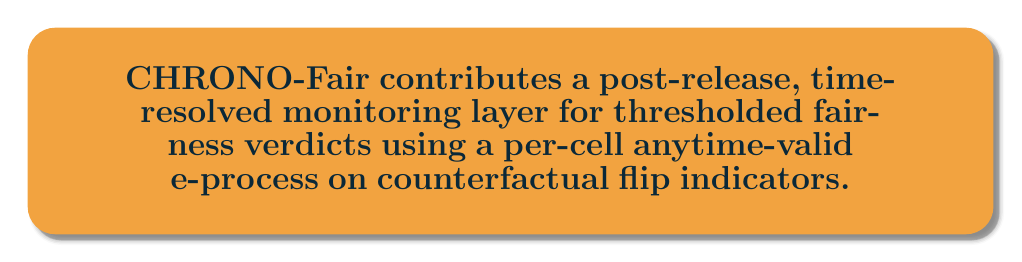
\begin{tikzpicture}
\node[fill=amber, text=ink, rounded corners=10pt, inner xsep=18pt, inner ysep=14pt,
       text width=11cm, align=center, drop shadow={blur shadow}] {%
\large \textbf{CHRONO-Fair contributes a post-release, time-resolved monitoring layer for thresholded fairness verdicts using a per-cell anytime-valid e-process on counterfactual flip indicators.}};
\end{tikzpicture}
\end{center}
\vfill
\centering\small
\textcolor{emerald}{\faIcon{eye}\, \textbf{Monitor, not mitigator}}\quad
\textcolor{amber}{\faIcon{play-circle}\, \textbf{Begins after Std~$\rightarrow$~Fair}}\\[4pt]
\textcolor{emerald}{\faIcon{cogs}\, \textbf{Agnostic to mitigation method}}\quad
\textcolor{amber}{\faIcon{flask}\, \textbf{Research prototype, not medical device}}
\vfill
\end{frame}
}

% ==========================================================
% Slide 7: Architecture
% ==========================================================
\begin{frame}{Planned architecture}
\centering
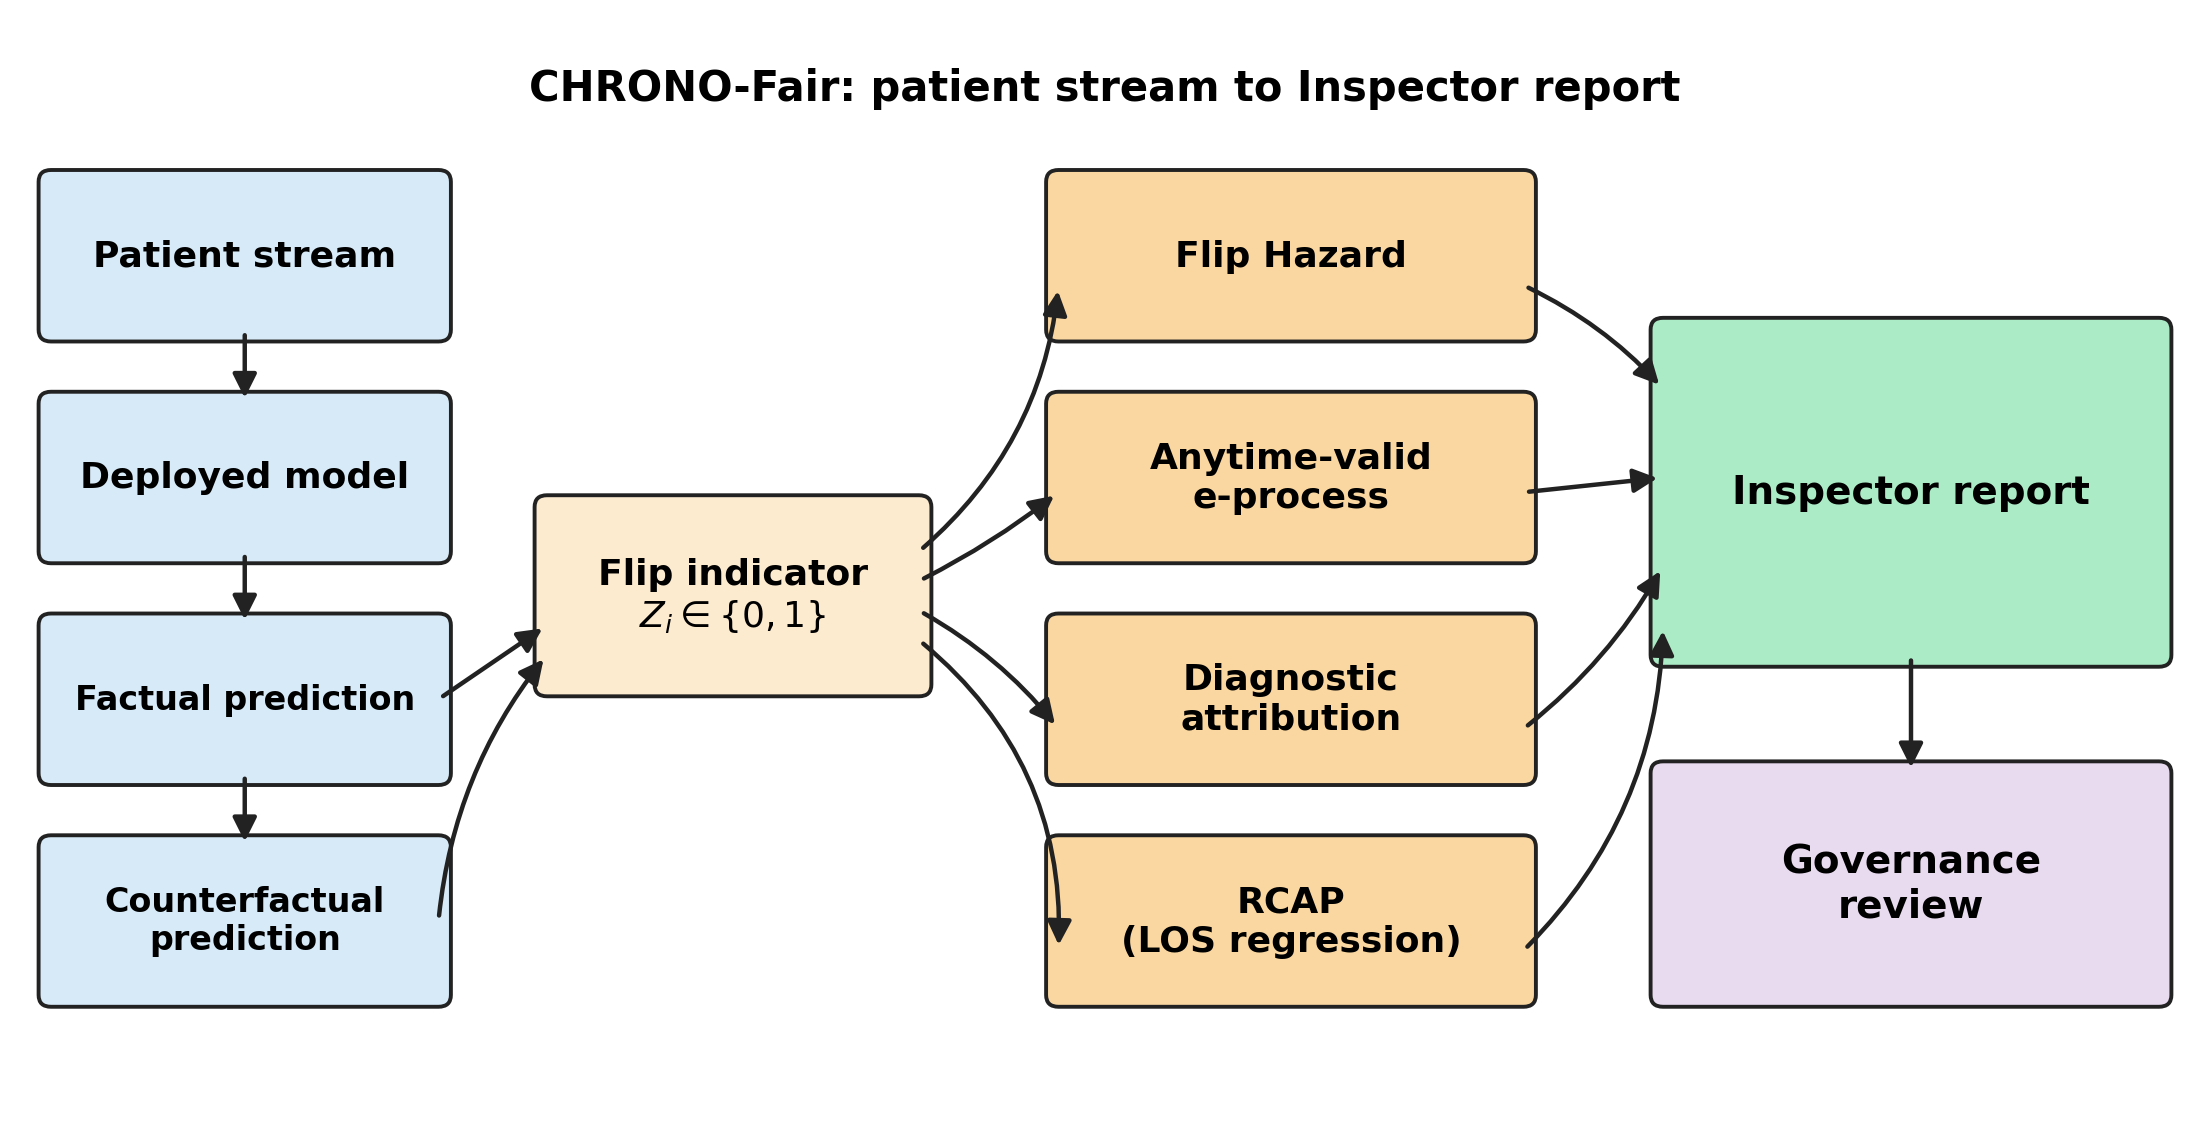
\includegraphics[width=0.93\linewidth]{../../chrono_fair_figures/fig0_architecture.png}\\
{\footnotesize\color{muted}\itshape Modules: Flip Hazard~[24]; per-cell shrunk-GROW e-process~[18, 19]; aleatoric/epistemic decomposition~[21]; RCAP Wasserstein-1 rank shift~[23].}
\end{frame}

% ==========================================================
% Slide 8: VFR-Audit to CHRONO-Fair
% ==========================================================
\begin{frame}{How CHRONO-Fair extends VFR-Audit}
\centering
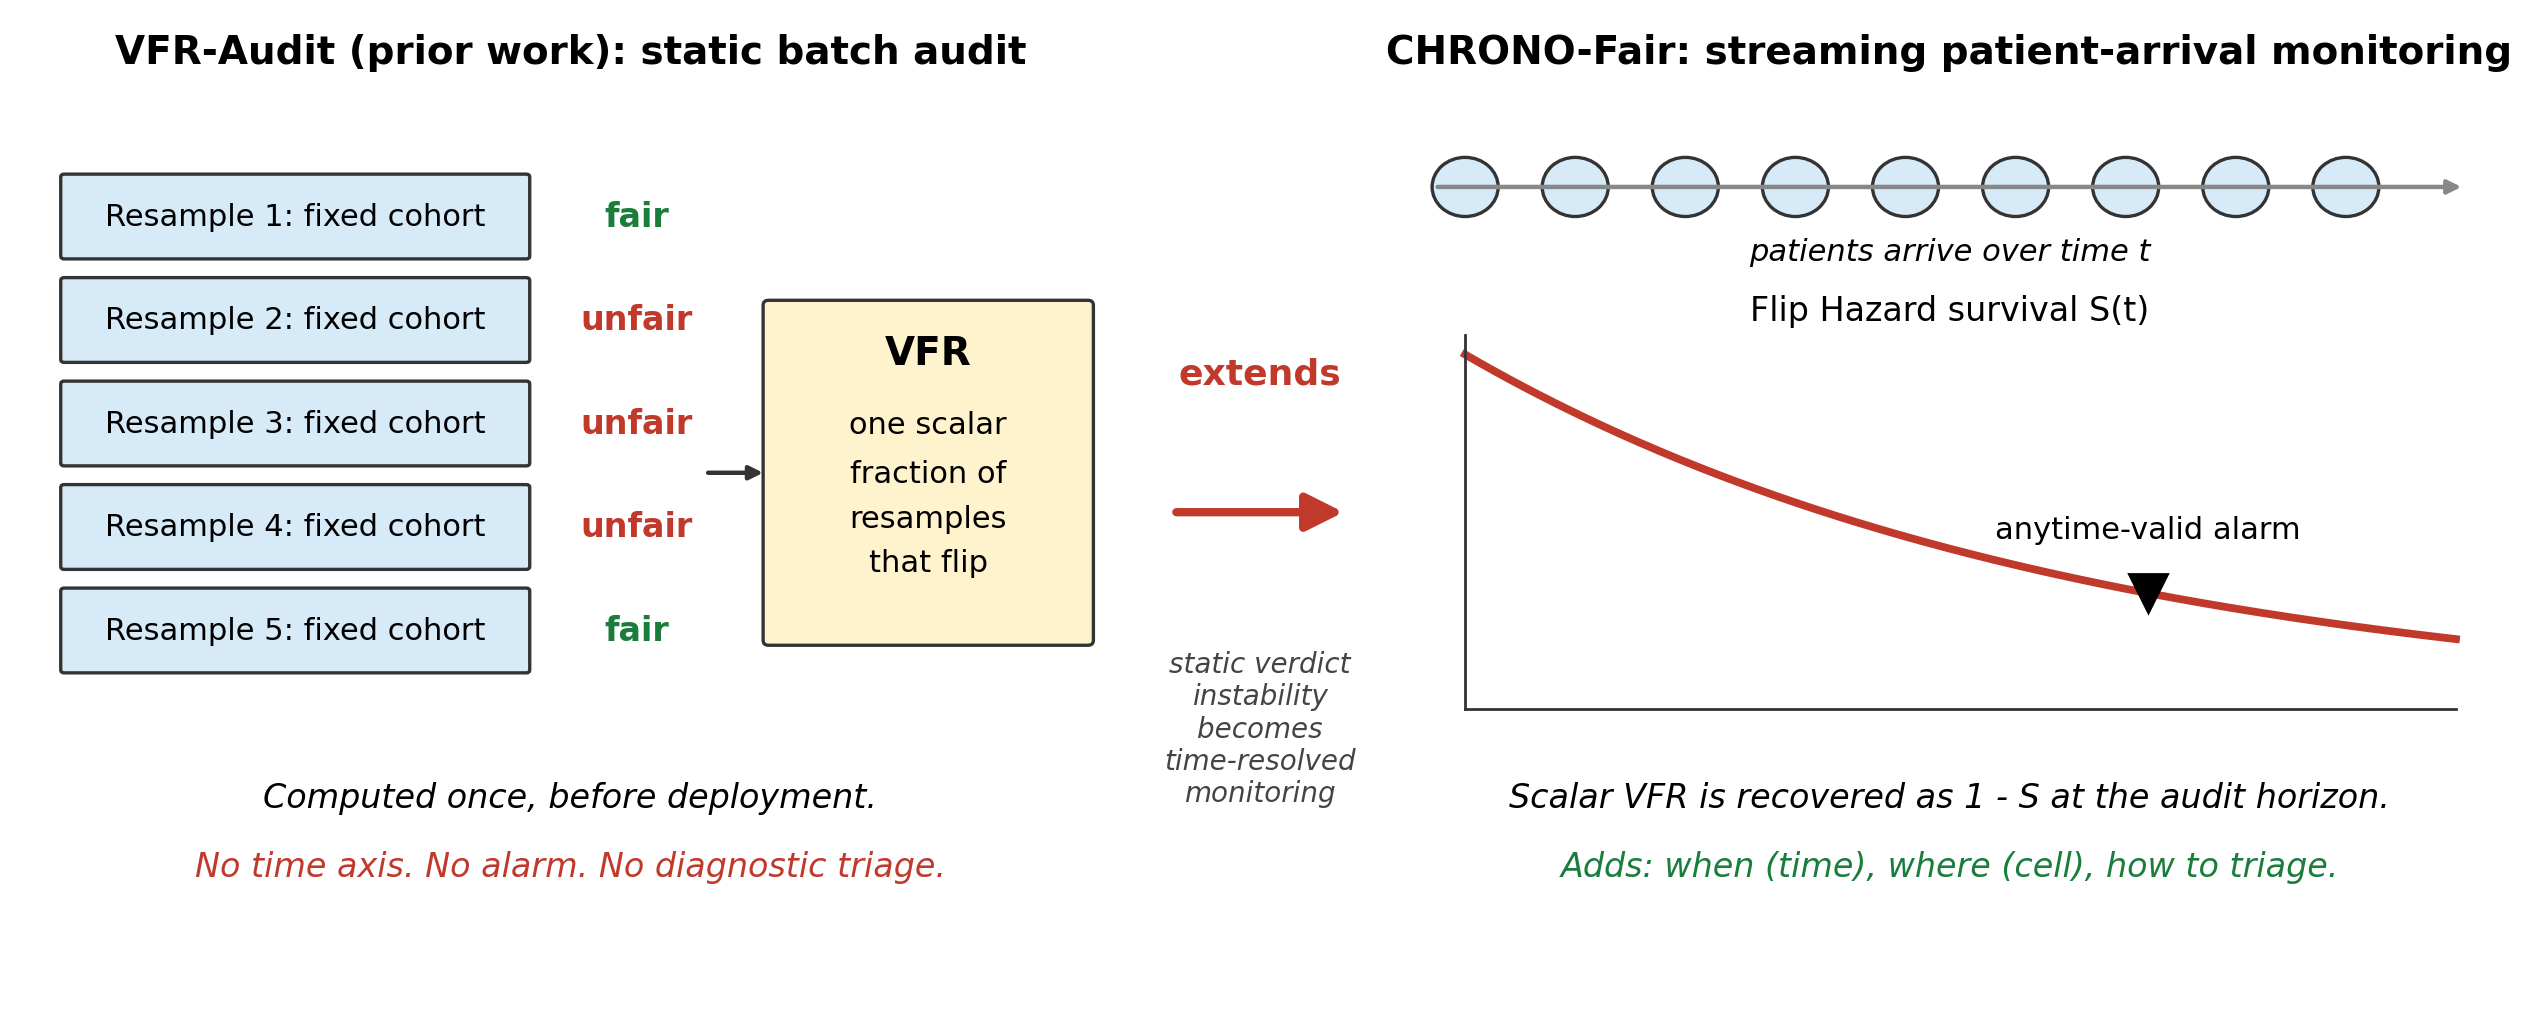
\includegraphics[width=\linewidth]{../../chrono_fair_figures/fig_concept_vfr_to_chrono.png}\\
{\footnotesize\color{muted}\itshape Scalar VFR is recovered as $1 - S$ at the audit horizon. CHRONO-Fair adds the time axis, the anytime-valid alarm rule, and the diagnostic triage signal.}
\end{frame}

% ==========================================================
% Slide 9: Mathematics attribution
% ==========================================================
\begin{frame}{Mathematics: \hfill \chip[soft]{what is taken vs what is ours}}
\scriptsize
\setlength{\arrayrulewidth}{0.6pt}\arrayrulecolor{rule}
\begin{tabular}{>{\bfseries}p{4.4cm} p{8.3cm}}
\toprule
\rowcolor{ink}
{\color{paper}\textbf{Equation / construct}} & {\color{paper}\textbf{Attribution}} \\
\midrule
Flip indicator $Z_i$ & \color{emerald}\textbf{Our definition}; same idea as prediction sensitivity~[22] \\
\rowcolor{soft}Flip Hazard $\lambda_a(t)$ & Standard hazard form (Kaplan-Meier~[24]; Nelson-Aalen 1972); \color{emerald}our naming and application \\
RMFT integral & Standard Restricted Mean Survival Time; adopted \\
\rowcolor{soft}e-process wealth $E_t$ & Waudby-Smith and Ramdas~[29]; Ramdas et al.~[20]; adopted \\
Shrunk GROW bet $\lambda_s$ & \color{emerald}\textbf{Our finite-sample shrinkage} of the GROW rule of~[29] \\
\rowcolor{soft}Ville's inequality (Thm.\ 1) & Ville 1939~[18]; standard application \\
Ensemble flip probability $\bar p^{\mathrm{flip}}$ & \color{emerald}\textbf{Our definition} \\
\rowcolor{soft}Aleatoric/epistemic entropy split & Depeweg et al.~[30]; Hullermeier and Waegeman~[21]; adopted \\
RCAP rank positions $u_i$ & Standard nonparametric group-conditional CDF; \color{emerald}our naming \\
\rowcolor{soft}RCAP $= W_1(\ldots)$ & Wasserstein-1 from optimal transport; adopted \\
\bottomrule
\end{tabular}
\vspace{4pt}\\
\textbf{\color{ink}The novelty is not a new survival estimator or a new e-process. The contribution is the coordinated integration of these instruments around the thresholded fairness verdict.}
\end{frame}

% ==========================================================
% Slide 10: Module-to-gap map
% ==========================================================
\begin{frame}{How each planned module closes one identified gap}
\centering\small
\begin{tikzpicture}[node distance=6pt]
\foreach \i/\gap/\mod/\desc in {%
  1/{Gap 1, time axis}/{Flip Hazard}/{Per-arrival survival curve instead of a single scalar [24].},%
  2/{Gap 2, peeking penalty}/{Per-cell anytime-valid e-process}/{Type-I control at every inspection step [18, 19, 20].},%
  3/{Gap 3, diagnostic interpretation}/{Aleatoric/epistemic decomposition}/{Triage label (data, model, mixed) per alarmed cell [21].},%
  4/{Gap 4, regression output}/{RCAP, Wasserstein-1 on ranks}/{Counterfactual rank shift for LOS regression [23].}%
} {
  \node[fill=amber, text=ink, rounded corners=4pt, minimum width=4.0cm, minimum height=0.9cm, align=center, font=\small\bfseries, text width=3.7cm] (gap\i) at (-7.0, -1.05*\i) {\gap};
  \node[font=\Large, text=emerald, right=2pt of gap\i] (arr\i) {\faIcon{angle-double-right}};
  \node[fill=soft, draw=emerald, line width=1pt, rounded corners=4pt, minimum width=8.5cm, minimum height=0.9cm, align=left, font=\small, text width=8.0cm, right=2pt of arr\i] (mod\i) {\textbf{\color{emerald}\mod.} \desc};
}
\end{tikzpicture}
\end{frame}

% ==========================================================
% Slide 11: Method discipline
% ==========================================================
\begin{frame}{Method discipline: \hfill \chip[coral]{what we will NOT claim}}
\small
\begin{itemize}\setlength\itemsep{4pt}
\item[\textcolor{emerald}{\faIcon{check-circle}}] \textbf{Per-cell anytime-valid Type-I control:} YES, under Ville inequality~[18, 19].
\item[\textcolor{coral}{\faIcon{times-circle}}] \textbf{Time-uniform online FDR:} NO. Step-wise BH is applied at inspection time only~[25, 26].
\item[\textcolor{coral}{\faIcon{times-circle}}] \textbf{Causal root cause:} NO. Diagnostic attribution is aleatoric/epistemic triage~[21].
\item[\textcolor{coral}{\faIcon{times-circle}}] \textbf{SCM-strength counterfactual:} NO. Feature-shift only; may under-flag indirect effects~[27, 28].
\item[\textcolor{coral}{\faIcon{times-circle}}] \textbf{Prospective clinical deployment:} NO. Controlled replay and simulation only.
\end{itemize}
\end{frame}

% ==========================================================
% Slide 12: Headline streaming result
% ==========================================================
\begin{frame}{Anchor streaming result \hfill \chip[soft]{controlled replay}}
\centering
\scriptsize
\setlength{\arrayrulewidth}{0.8pt}\arrayrulecolor{rule}
\begin{tabular}{>{\bfseries}l c c}
\toprule
\rowcolor{ink}
{\color{paper}\textbf{Method}} & {\color{paper}\textbf{Detected}} & {\color{paper}\textbf{Mean delay (patients)}} \\
\midrule
\rowcolor{soft} CHRONO-Fair (per-cell e-process) & \textcolor{emerald}{\textbf{50 / 50}} & \textcolor{emerald}{\textbf{837 (median 828)}} \\
ADWIN ($k = 1$)                  & 21 / 50 & 3\,878 \\
\rowcolor{soft} ADWIN ($k = 25$)            & 21 / 50 & 3\,927 \\
Davis-style ADWIN on fairness gap & 21 / 50 & 3\,904 \\
\rowcolor{soft} Periodic batch ($n = 500$) & 24 / 50 & 499 (no peeking control) \\
Static VFR                        & 0 / 50 & \textendash \\
\bottomrule
\end{tabular}
\vspace{6pt}\\
{\footnotesize\color{muted}\itshape 10\,000-patient stream, drift onset at 5\,000, 50 Monte-Carlo runs. False-alarm rate at or below the nominal $\alpha$ for every tested $\alpha$~[19, 29].}\\
{\footnotesize\color{coral}\textbf{Streaming evidence is controlled replay and simulation. Not prospective clinical validation.}}
\end{frame}

% ==========================================================
% Slide 13: Phased plan
% ==========================================================
\begin{frame}{Plan: how the gap will actually be closed}
\small
\begin{itemize}\setlength\itemsep{4pt}
\item[\chip[amber]{Phase 1}] \textbf{Controlled-validation evidence.} Real Texas-100X batch + Texas-100X-calibrated streaming/replay + robustness stress tests.\\
  \textcolor{muted}{\itshape Status: drafted, in revision for Q1 submission.}
\item[\chip[amber]{Phase 2}] \textbf{Methodological strengthening.} Time-uniform online FDR~[25, 26]; SCM counterfactual sensitivity~[27, 28].\\
  \textcolor{muted}{\itshape Status: planned for next revision.}
\item[\chip[amber]{Phase 3}] \textbf{Prospective evaluation.} Site-partnered EHR-stream validation; governance-user evaluation.\\
  \textcolor{muted}{\itshape Status: scoping, partner search.}
\item[\chip[amber]{Phase 4}] \textbf{Artifact release.} Anonymised proof-of-concept prototype + configs + seeds + scripts.\\
  \textcolor{muted}{\itshape Status: scheduled for camera-ready.}
\end{itemize}
\end{frame}

% ==========================================================
% Slide 14: Asks
% ==========================================================
\begin{frame}{Asks for this meeting}
\small
\begin{enumerate}\setlength\itemsep{3pt}
\item Is the post-release monitoring framing the right contribution to lead with, vs a methods-only framing of the per-cell e-process?
\item Is the Std/Fair monitored-model table (cited from prior VFR-Audit study) acceptable as the predecessor without re-running it?
\item Which Q1 venue is best: Frontiers in Digital Health, npj Digital Medicine, JAMIA, JBI, or NEJM AI?
\item Should I add a second real cohort (MIMIC-IV / eICU) before submission, or submit single-dataset with a prospective-validation roadmap?
\item Defer artifact release to camera-ready, or supply a minimum-viable artifact preview at submission?
\item Timing: next-round submission in 6 to 8 weeks, or invest 2 to 3 months in Phase 2 strengthening first?
\end{enumerate}
\end{frame}

% ==========================================================
% Slide 15-17: References
% ==========================================================
\begin{frame}[allowframebreaks]{References}
\scriptsize
\begin{enumerate}
\item Wong et al. External validation of a sepsis prediction model. JAMA Intern.\ Med., 2021.
\item Davis et al. Quarterly subgroup-performance drift in a deployed VA model. npj Digital Medicine, 2025.
\item Obermeyer et al. Dissecting racial bias in a care-management algorithm. Science, 2019.
\item Seyyed-Kalantari et al. Underdiagnosis bias of AI in chest X-ray. Nature Medicine, 2021.
\item Vyas et al. Hidden in plain sight: race-based clinical algorithms. NEJM, 2020.
\item Habib et al. External validation of the Epic Sepsis Model. JAMA Network Open, 2021.
\item U.S.\ FDA. Predetermined Change Control Plan for AI/ML-enabled device software functions, 2024.
\item European Parliament and Council. Regulation (EU) 2024/1689 (EU AI Act), 2024.
\item Vasey et al. DECIDE-AI reporting guideline. Nature Medicine, 2022.
\item Collins et al. TRIPOD+AI statement. BMJ, 2024.
\item Liu et al. CONSORT-AI. Nature Medicine, 2020.
\item Alderman et al. STANDING Together consensus. Lancet Digital Health, 2025.
\item Saleiro et al. Aequitas, 2018.
\item Bird et al. Fairlearn, 2020.
\item Bellamy et al. AI Fairness 360. IBM J.\ R\&D, 2019.
\item Microsoft Responsible AI Dashboard, 2022.
\item Authors (anonymised). VFR-Audit prior work; cited in third person.
\item Ville. Etude critique de la notion de collectif, 1939.
\item Howard et al. Time-uniform confidence sequences. Annals of Statistics, 2021.
\item Ramdas et al. Game-theoretic statistics. Statistical Science, 2023.
\item Hullermeier and Waegeman. Aleatoric and epistemic uncertainty. Machine Learning, 2021.
\item Maughan and Near. Prediction sensitivity, 2022.
\item Cherian and Candes. Statistical inference for fairness auditing. JMLR, 2024.
\item Kaplan and Meier. Nonparametric estimation from incomplete observations. JASA, 1958.
\item Javanmard and Montanari. Online FDR control. Annals of Statistics, 2018.
\item Benjamini and Hochberg. Controlling the false discovery rate. JRSS-B, 1995.
\item Kusner et al. Counterfactual fairness. NeurIPS, 2017.
\item Chiappa. Path-specific counterfactual fairness. AAAI, 2019.
\item Waudby-Smith and Ramdas. Estimating means by betting. JRSS-B, 2024.
\item Depeweg et al. Decomposition of uncertainty for active learning. ICML, 2018.
\end{enumerate}
\end{frame}

\end{document}
